%! suppress = UnresolvedReference


\chapter{\app 的设计}\label{ch:design}


\section{应用的整体架构设计}\label{sec:arch-design}

本应用的整体架构如图~\ref{fig:model} 所示。因空间有限,此处对部分模块进行了合并与省略,后续小节会展开介绍。

\begin{figure}[!ht]
    \centering
    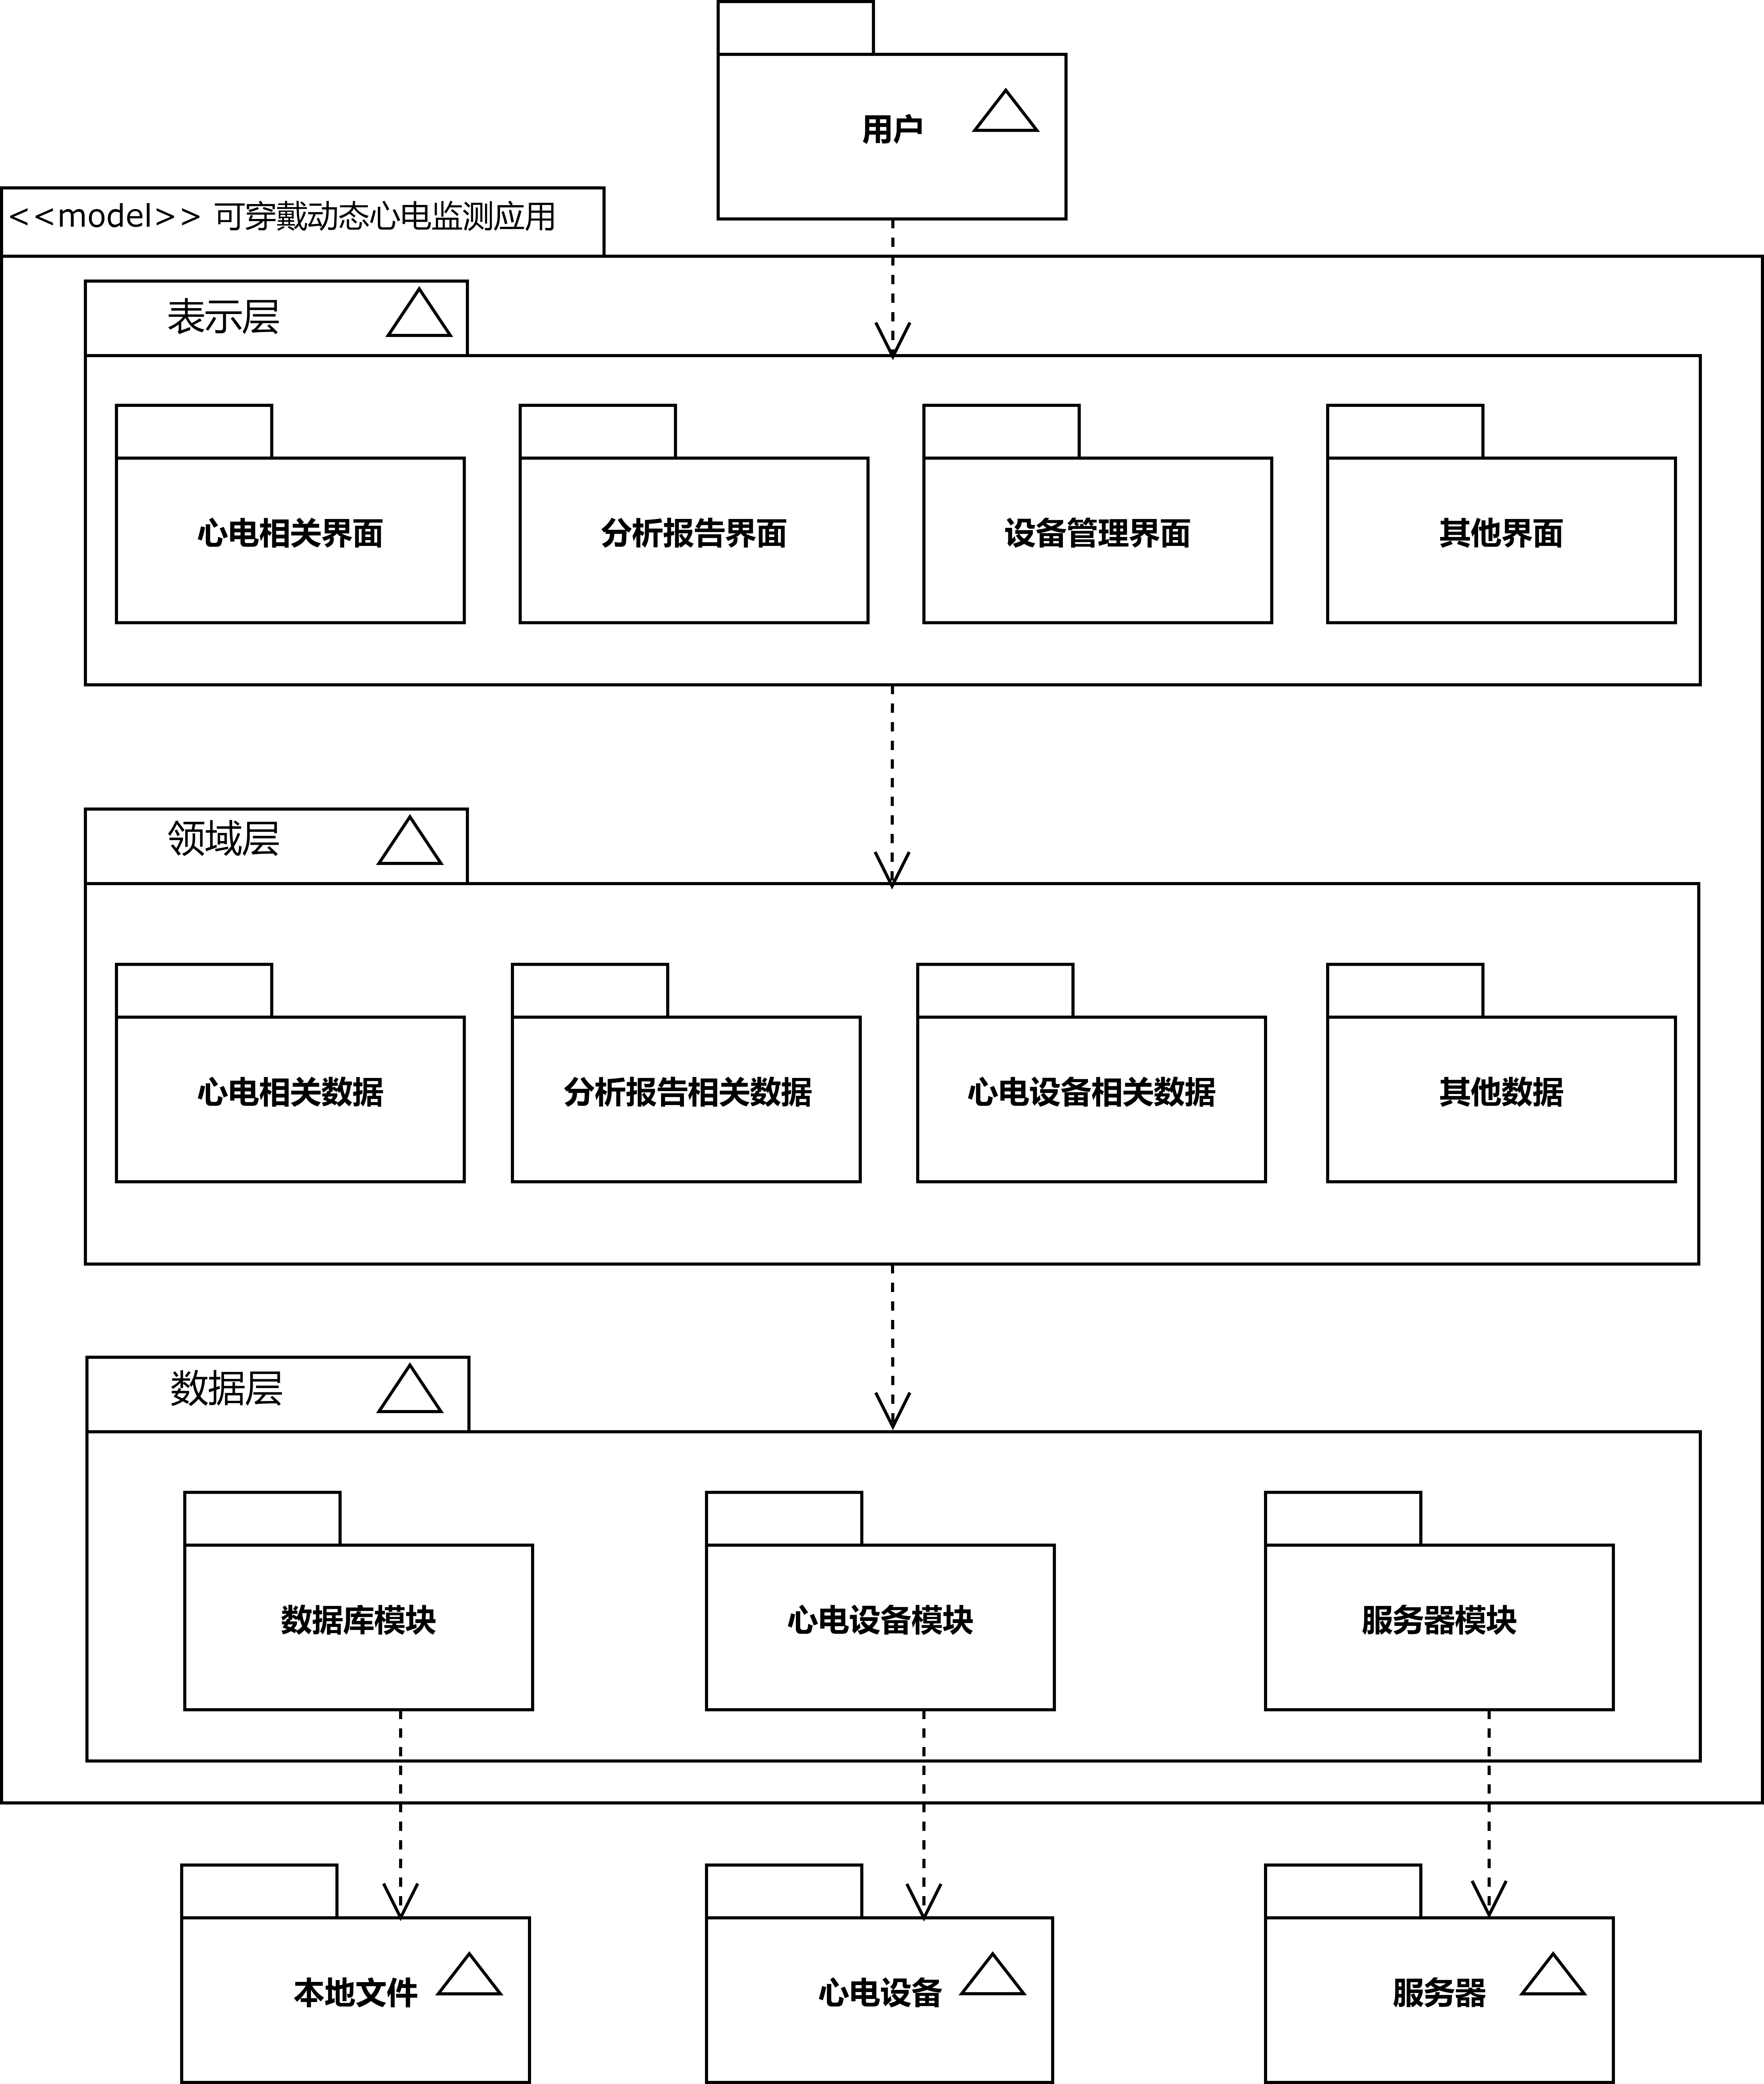
\includegraphics[width=.9\textwidth]{../assets/model.drawio}
    \bicaption{应用的整体架构}{Architecture of the app}
    \label{fig:model}
\end{figure}

本应用使用了Riverpod架构模式\cite{bizzottoFlutterAppArchitecture},其与MVC等传统模式有较大差别,且由于提出较晚而知名度不高,因此本节顺带对该模式进行简单介绍。

在设计应用程序时选择正确的应用架构至关重要,过于简陋的设计会使得代码整体缺乏组织性,过于繁复的设计则会阻碍代码的修改迭代。自最经典的MVC架构以来,已有许多流行的应用架构被相继提出。其中一些对原始的MVC架构进行改动后仍沿用其名称,导致MVC这一术语的含义愈加模糊;另一些变体则被命名为MVP、MVVM、MVC+S等MV*,或是如Clean Architecture等另起炉灶。这些经典的架构模式很难原样照搬至Flutter框架,即使强行在Flutter中进行实现也只会使得代码结构不伦不类。在探索Flutter适用的应用架构的过程中,社区已经提出了许多新模式,如BLoC、Stacked等。而在本应用的架构设计中,采用的则是Andrea于2022年初提出的Riverpod架构模式。

Flutter曾经有一个流行的状态管理包Provider,该包也是上述的BLoC、Stacked等架构模式的基础。后来,由于Provider包的设计逐渐暴露出一些难以解决的问题,其开发者将该包进行了大幅重写,并因其与旧版本不兼容而改名为Riverpod(对Provider中字母的重组)重新发布,Andrea提出的该架构模式因基于Riverpod包而命名为Riverpod架构模式。

该架构模式由三层或四层组成,从上至下分别是表示(Presentation)层、可选的应用(Application)层、领域(Domain)层、数据(Data)层。

\subsection{表示层}\label{subsec:presentation-layer}

表示层类似于MVC中的View和Controller,或是MVVM中的View和ViewModel,以及Android应用架构指南\footnote{\url{https://developer.android.com/jetpack/guide\#recommended-app-arch}}中的UI层。该层包含用户可见的UI组件以及相关的特定于某个组件的状态与交互逻辑。由于Flutter采用了响应式的设计思想,UI本身与其对应的状态的关系极为密切,因此在Riverpod架构中,将MV*中的Model以外的两层进行了合并。在本应用中,该层包含实时心电界面、历史心电界面、分析报告界面等内容。

\subsection{应用层}\label{subsec:app-layer}

应用层类似Android应用架构指南中的领域层(两边对领域层这一术语的使用不一致),并且与其一样是可选的。这是因为并非所有应用都具有复杂的业务逻辑,也并非所有业务逻辑都需要被提取出来以便重用。在Riverpod架构中,如果不需要应用层,则可以直接省略这一层。在本应用中,由于应用的业务逻辑较为简单,因此并未使用该层。

\subsection{领域层}\label{subsec:domain-layer}

领域层类似于MV*中的Model。该层包含领域模型,即应用程序中的数据及其相关的方法。由于领域层在各种架构模式中被广泛使用(尽管命名可能不同),此处不作详细介绍。在本应用中,该层包括心电数据、心拍数据、应用设置数据等模型。

\subsection{数据层}\label{subsec:data-layer}

数据层类似Android应用架构指南中的数据层。该层包含与外部数据源通信的相关代码,负责将领域模型与底层的数据源的实现细节进行隔离,将从数据源获取的原始格式的数据(如JSON等)转换为领域层中的领域对象(应用中自定义的数据类),有时也执行数据缓存等操作。在本应用中,该层包含与数据库、心电监测设备、服务器进行通信的相关代码。


\section{应用各个模块的设计}\label{sec:app-design}

\subsection{心电模块的设计}\label{subsec:ecg-design}

心电模块的整体架构如图~\ref{fig:model-ecg} 所示。因Riverpod架构模式未指明外部函数接口和后台定时任务属于哪一层,本图将其绘制于已有层次之外。

\begin{figure}[!ht]
    \centering
    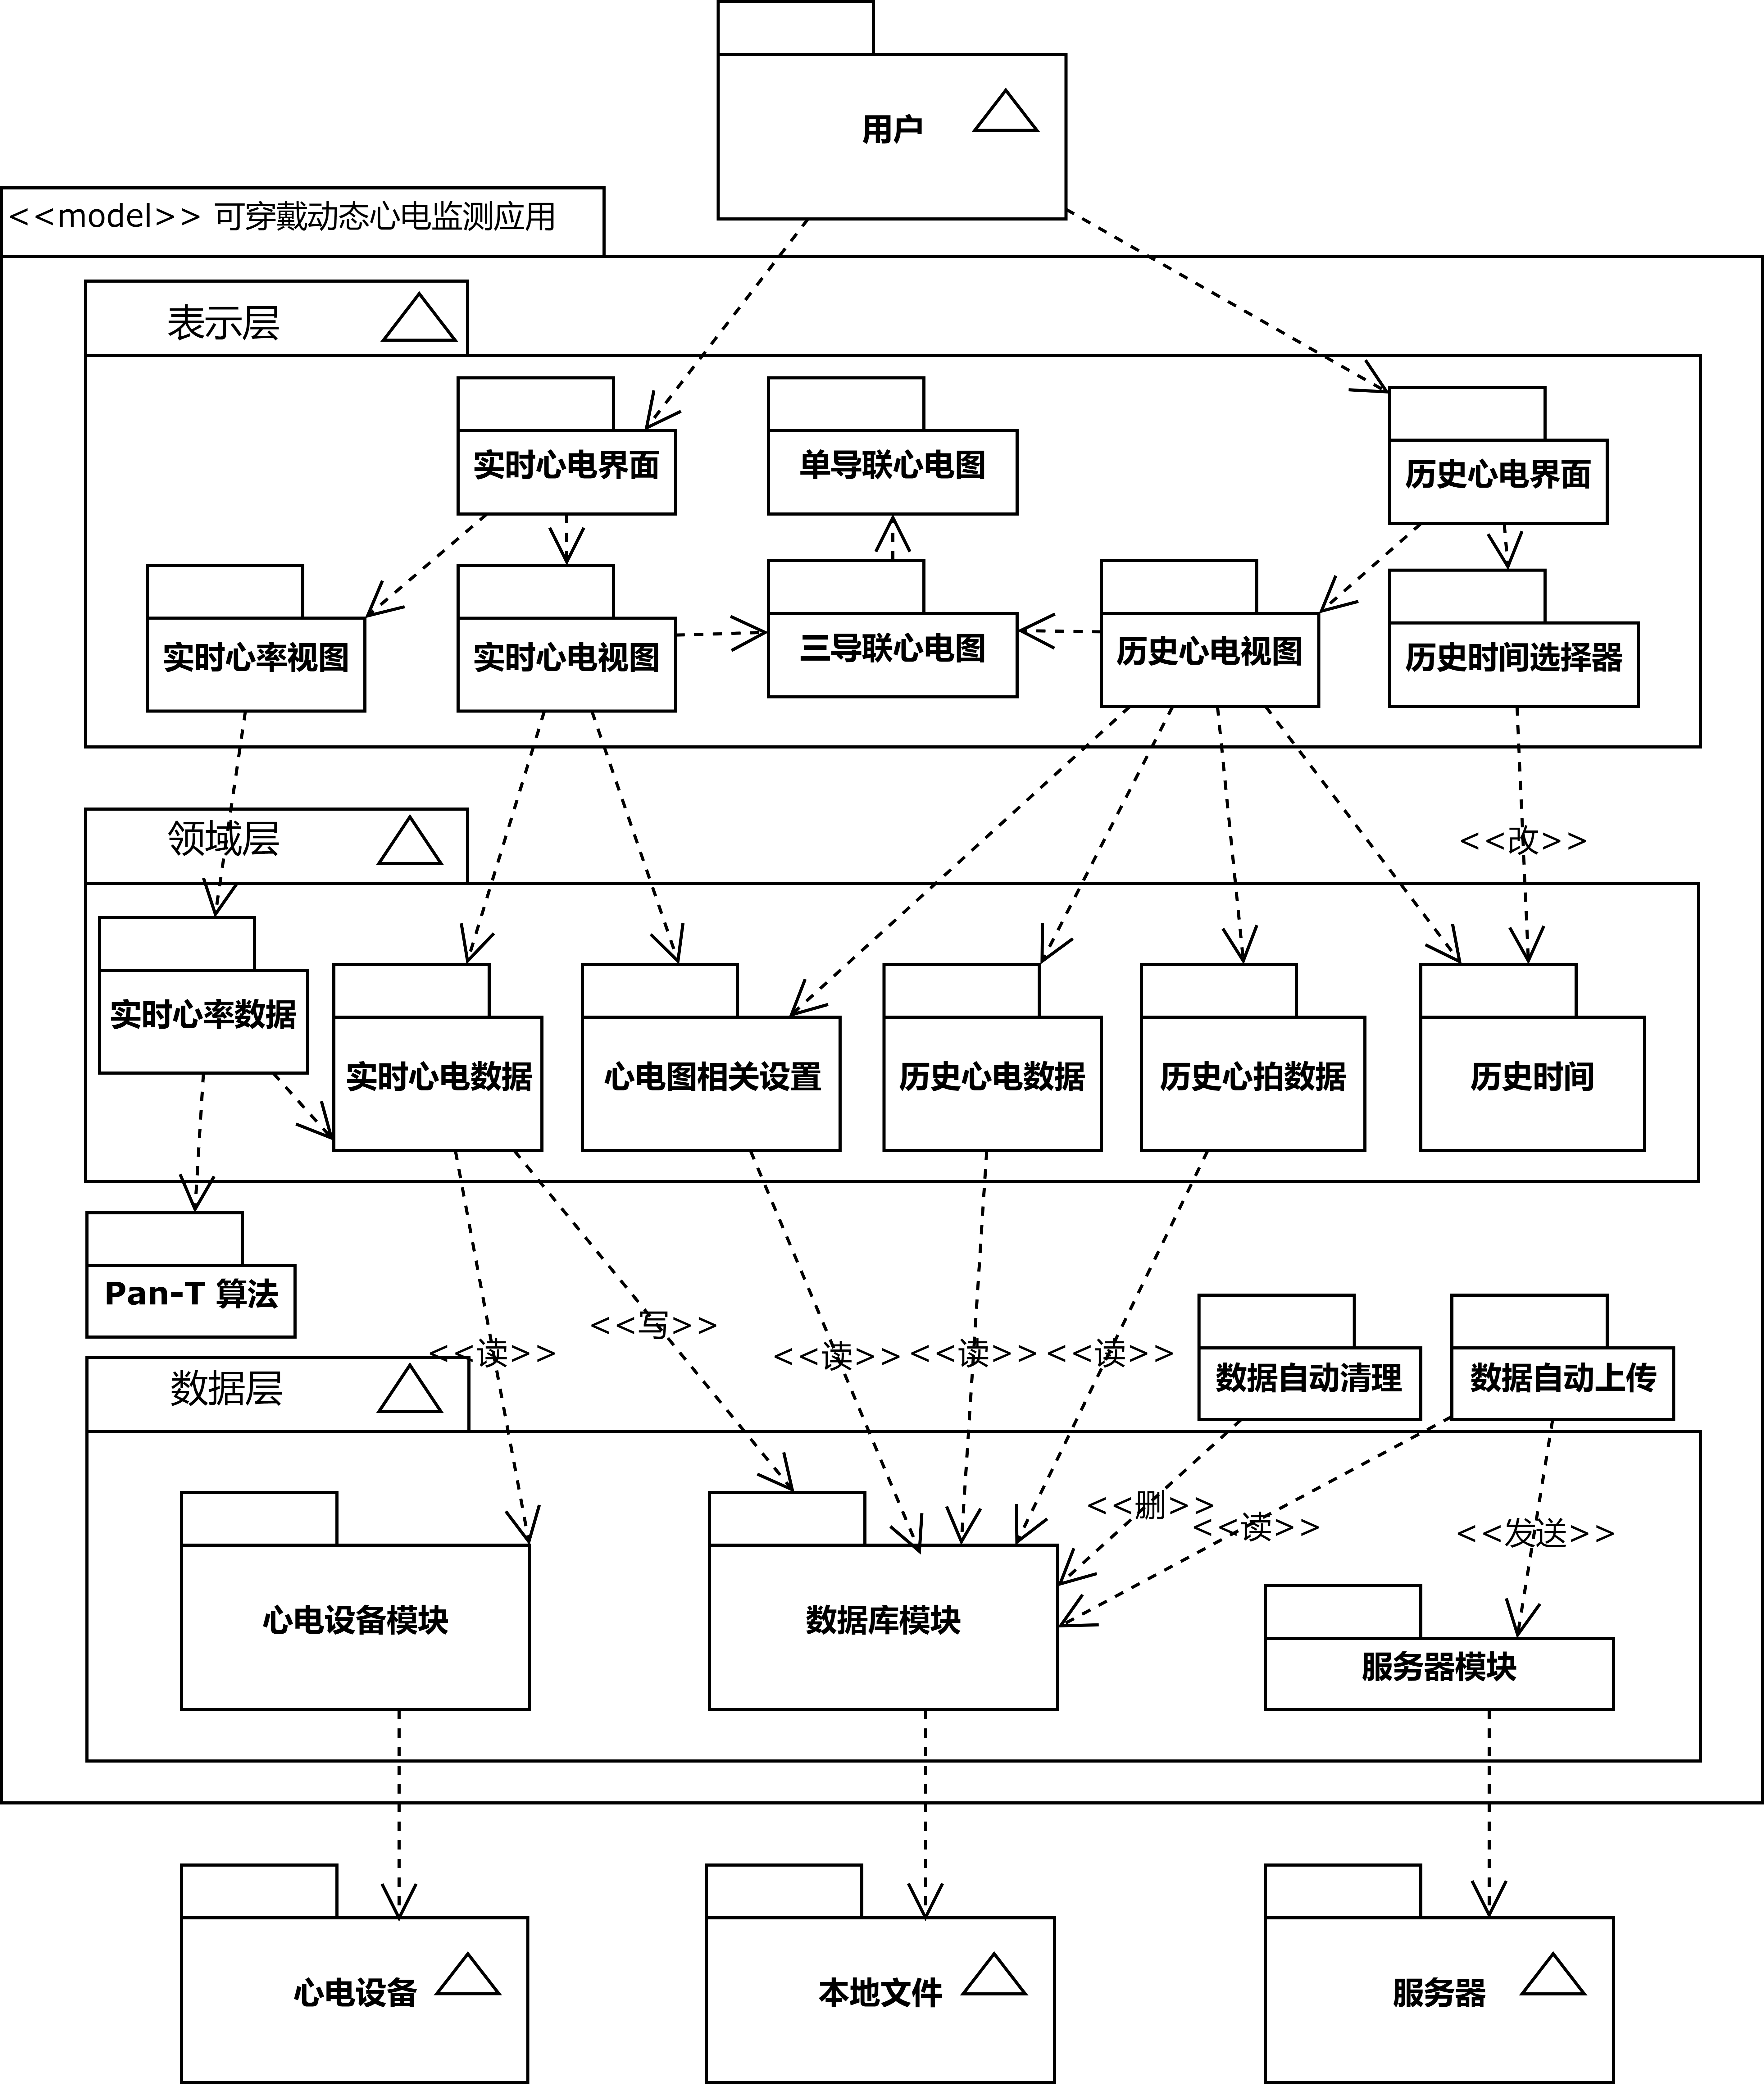
\includegraphics[width=.8\textwidth]{../assets/model-ecg.drawio}
    \bicaption{心电模块的架构}{Architecture of the ECG module}
    \label{fig:model-ecg}
\end{figure}

心电模块可以大致划分为实时心电模块和历史心电模块这两个子模块,不过两者在各个层级的重合部分较多,在最终的实现中也有不少共享的代码,因此一并归于心电模块。

\subsubsection{表示层}

心电模块的表示层中为用户提供了两个心电相关的界面,分别是实时心电界面和历史心电界面。实时心电界面包含实时心电视图和实时心率视图,历史心电界面则包含历史心电视图和历史时间选择器。实时心电视图与历史心电视图均为心电图的显示,因此提取其共享部分作为三导联心电图UI组件。然后,由于三个导联的心电图之间也高度相似,在三导联心电图之中再提取出单导联心电图UI组件,以免编写重复代码。

\subsubsection{领域层}

心电模块的领域层中,实时心率数据由实时心率视图读取;实时心电数据由实时心电视图读取,也被用于心率数据的获取,并被存入数据库;心电图相关设置数据由实时心电视图和历史心电视图读取(实际上有不同的设置项,但在该设计层次无须细分);历史心电数据和历史心拍数据由历史心电视图读取;历史时间由历史时间选择器进行修改,由历史心电视图读取,并被用于对历史心电数据和历史心拍数据的查询。

\subsubsection{其他层}

Pan-Tompkins算法(图中简写为Pan-T算法)模块以C++语言实现,通过Dart FFI被调用,用于通过实时心电数据得到心拍位置,进而得到心率数据;另外,Pan-Tompkins算法所给出的心拍位置也会作为未知类型的心拍存入数据库,以供历史时间选择器使用(跳转至上一个或下一个心拍的时间),为了保证图像清晰而并未在图中标出。数据自动清理模块和数据自动上传模块都是后台定时运行的自动任务,对用户而言并不可见;数据自动清理模块负责清理较旧的数据,避免应用占用空间过多;数据自动上传模块负责将数据库中的数据上传至服务器作为备份。

\subsubsection{数据层}

心电模块需要用到数据层中的所有三个子模块。心电设备模块用于提供实时心电数据;数据库模块用于实时心电数据的写入、心电相关设置与历史心电数据的读取、来源于Pan-Tompkins算法的心拍位置的写入、历史心拍数据的读取;服务器模块用于数据上传。

\subsection{分析报告模块的设计}\label{subsec:analytics-design}

分析报告模块的整体架构如图~\ref{fig:model-analytics} 所示。

\begin{figure}[!ht]
    \centering
    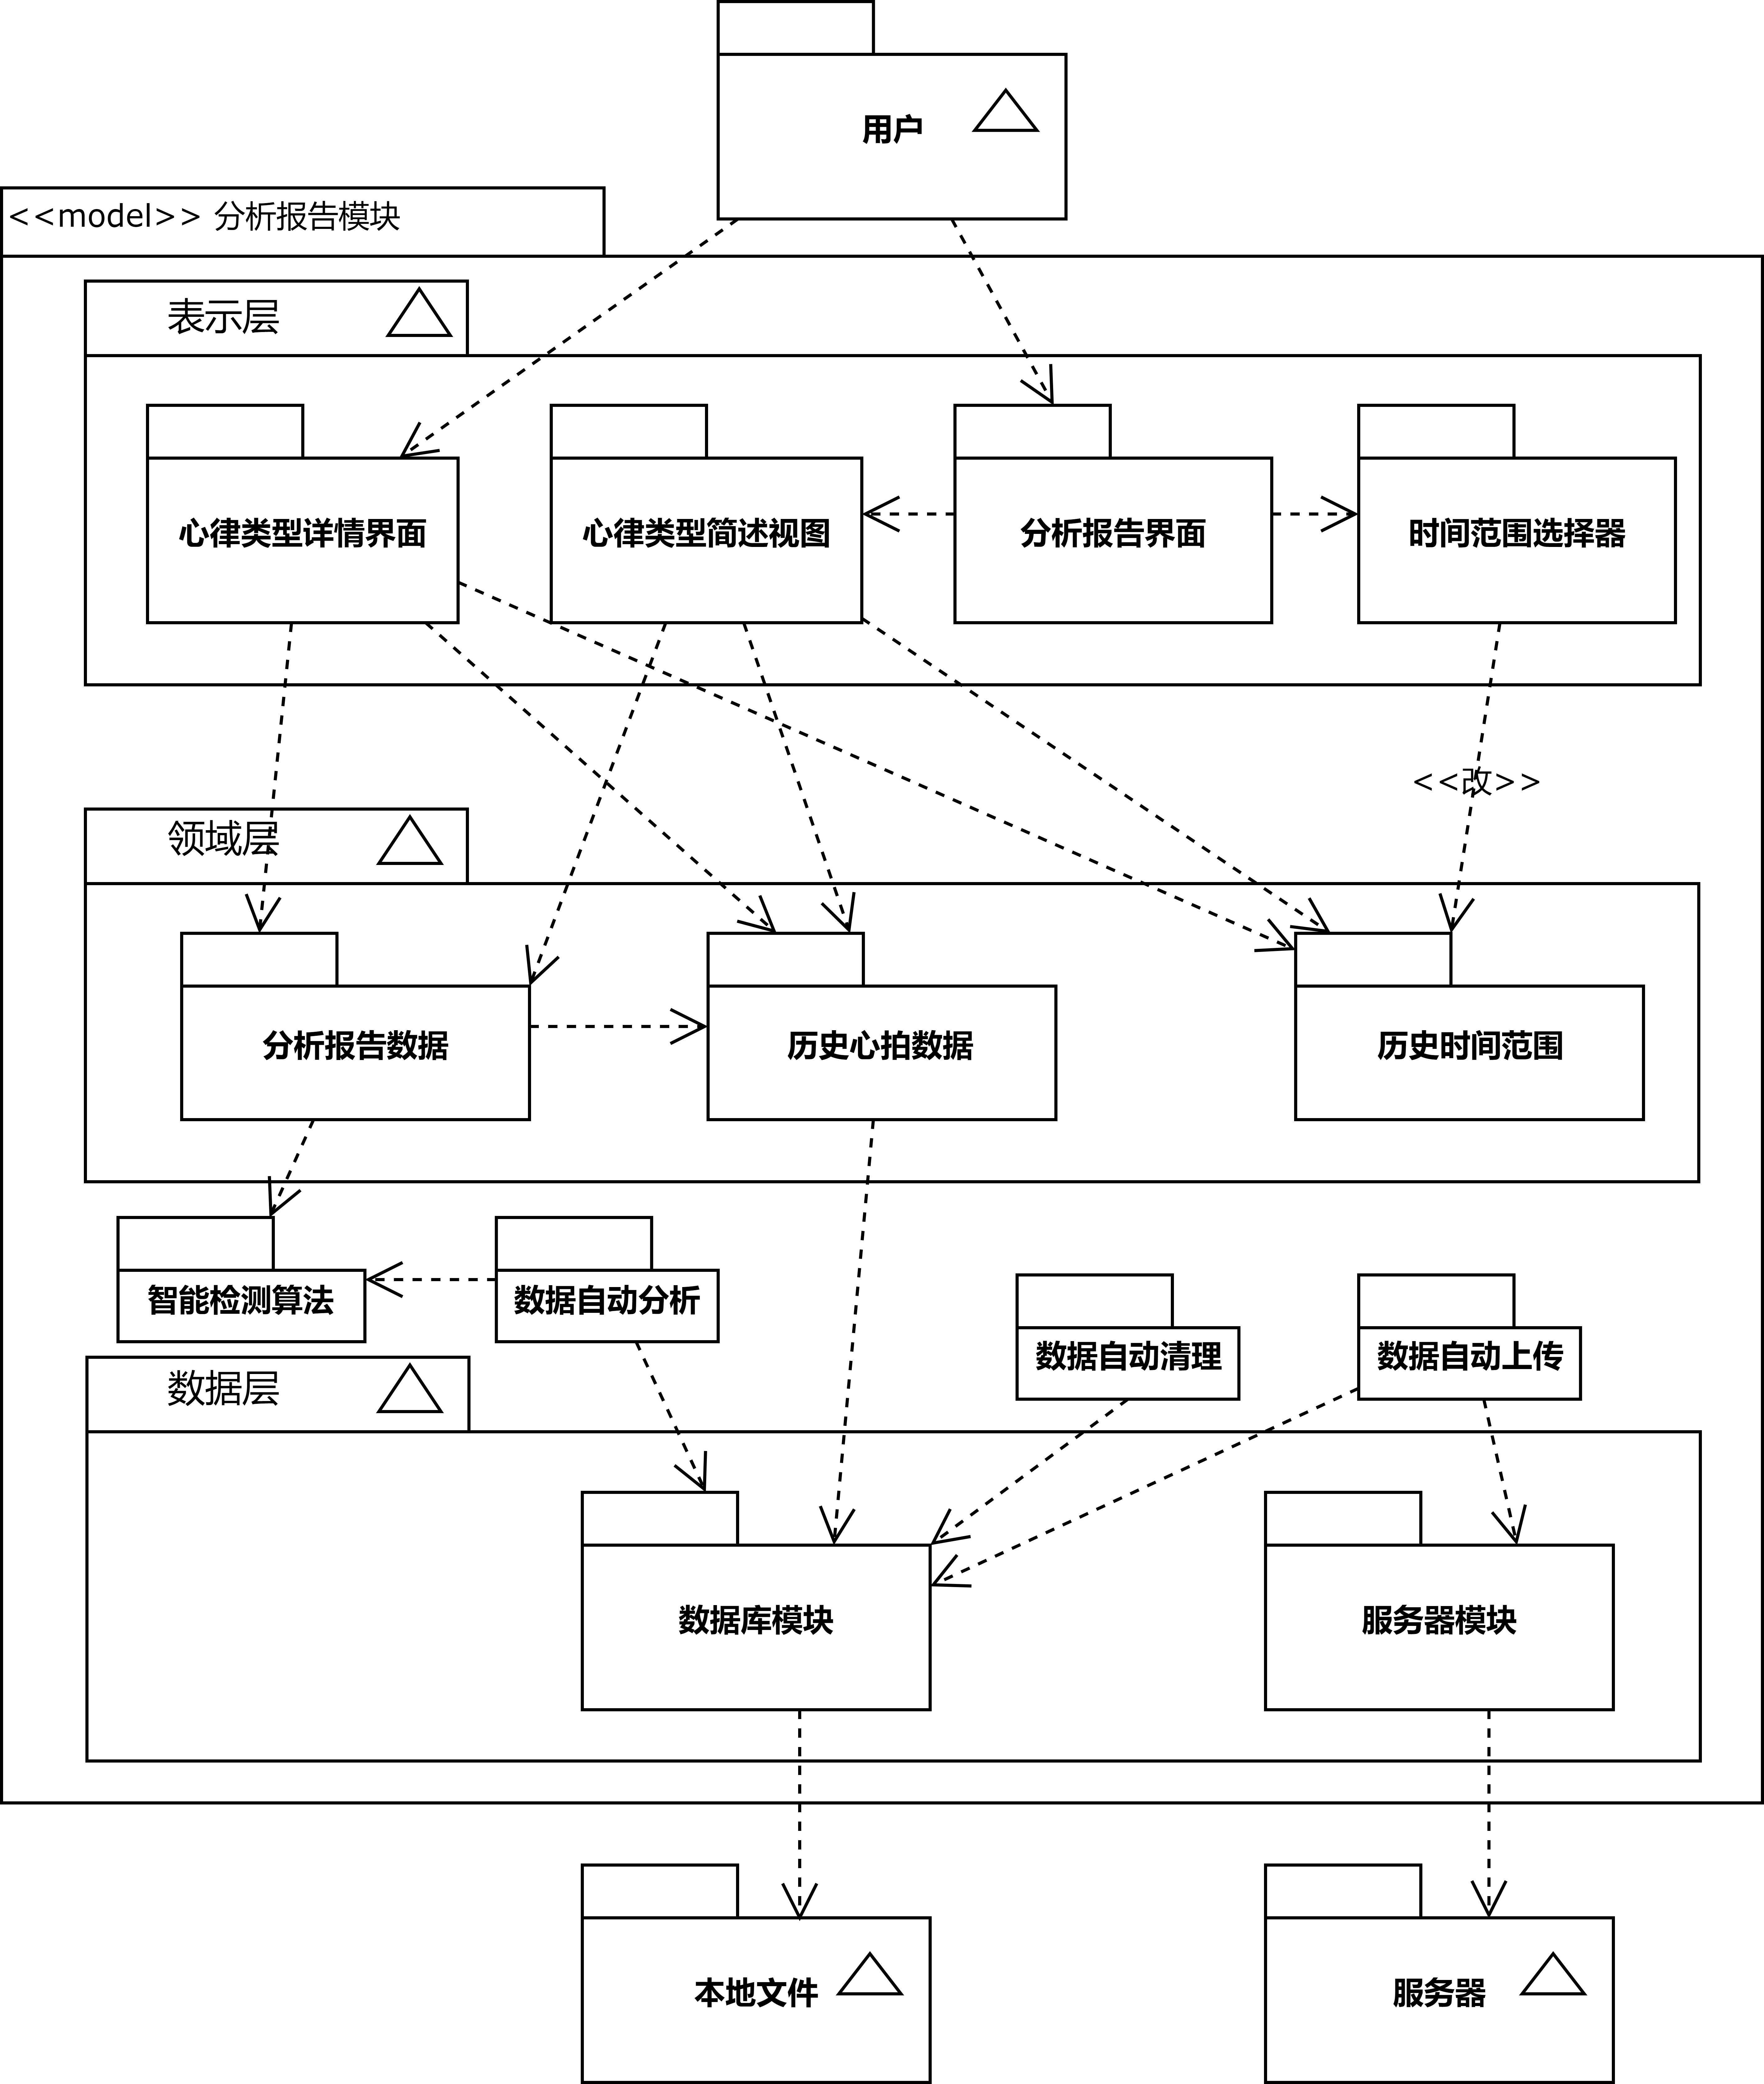
\includegraphics[width=.8\textwidth]{../assets/model-analytics.drawio}
    \bicaption{分析报告模块的架构}{Architecture of the analytics module}
    \label{fig:model-analytics}
\end{figure}

\subsubsection{表示层}

分析报告模块的表示层包含两个界面,分别是分析报告界面和心律类型详情界面。分析报告界面用于展示对各个心律类型的分析结果的总结,包含心律类型简述视图和用于控制分析时间段的时间范围选择器。点击某个心律类型简述视图所在区域后,会打开心律类型详情界面,详细说明该心律类型的情况,包括该心律类型每次出现的时间,点击时间可以跳转至历史心电界面的对应时间。

\subsubsection{领域层}

分析报告模块的领域层包含三个数据模型,分别是分析报告数据、历史心拍数据和历史时间范围。三个数据都同时被心律类型简述视图和心律类型详情界面所读取,因为前者只是后者的折叠形式。历史时间范围还被时间范围选择器展示和设置。历史时间范围即当前所查看的分析报告包含的时间范围,被读取后用于历史心拍数据的查询参数。历史心拍数据即过去的每个心拍的位置和对应的心律类型。分析报告数据是基于历史心拍数据的分析结果,比如平均心室率等。

\subsubsection{其他层}

数据自动清理模块和数据自动上传模块与历史心电中的作用相同,不进行重复说明。数据自动分析模块每10分钟自动运行一次(这是所用模型允许的最短输入数据的时长),读取过去10分钟的历史心电数据,输入智能检测算法,将得到的心拍分类结果写入数据库。该算法在后台自动运行,而非延迟到用户查询分析报告时再运行,原因之一是为了能将分析结果及时上传至服务器;原因之二是分析每10分钟的数据需要数秒时间,虽然不长,但用户选取较长范围时仍需要一定时间的等待,提前分析并存入数据库可以作为缓存;原因之三是历史心拍数据比较容易裁切和拼接,方便分段存入数据库和进行任意时间段的查询。而基于历史心拍数据分析得到的分析报告数据则因为计算量小而没有必要预先缓存,且较难进行多时间段的拼接和分离,因此在用户查询分析报告时才进行分析。

\subsubsection{数据层}

分析报告模块需要用到数据层中的数据库模块和服务器模块。数据库模块用于历史心电数据的查询、历史心拍数据的写入与查询。服务器模块用于数据上传。心电设备模块在分析报告模块中并不需要,用户甚至可以在已经断开心电监测设备的连接时查看分析报告,并不会对本模块的功能产生影响。

\subsection{设备管理模块的设计}\label{subsec:device-design}

设备管理模块的整体架构如图~\ref{fig:model-device} 所示。

\begin{figure}[!ht]
    \centering
    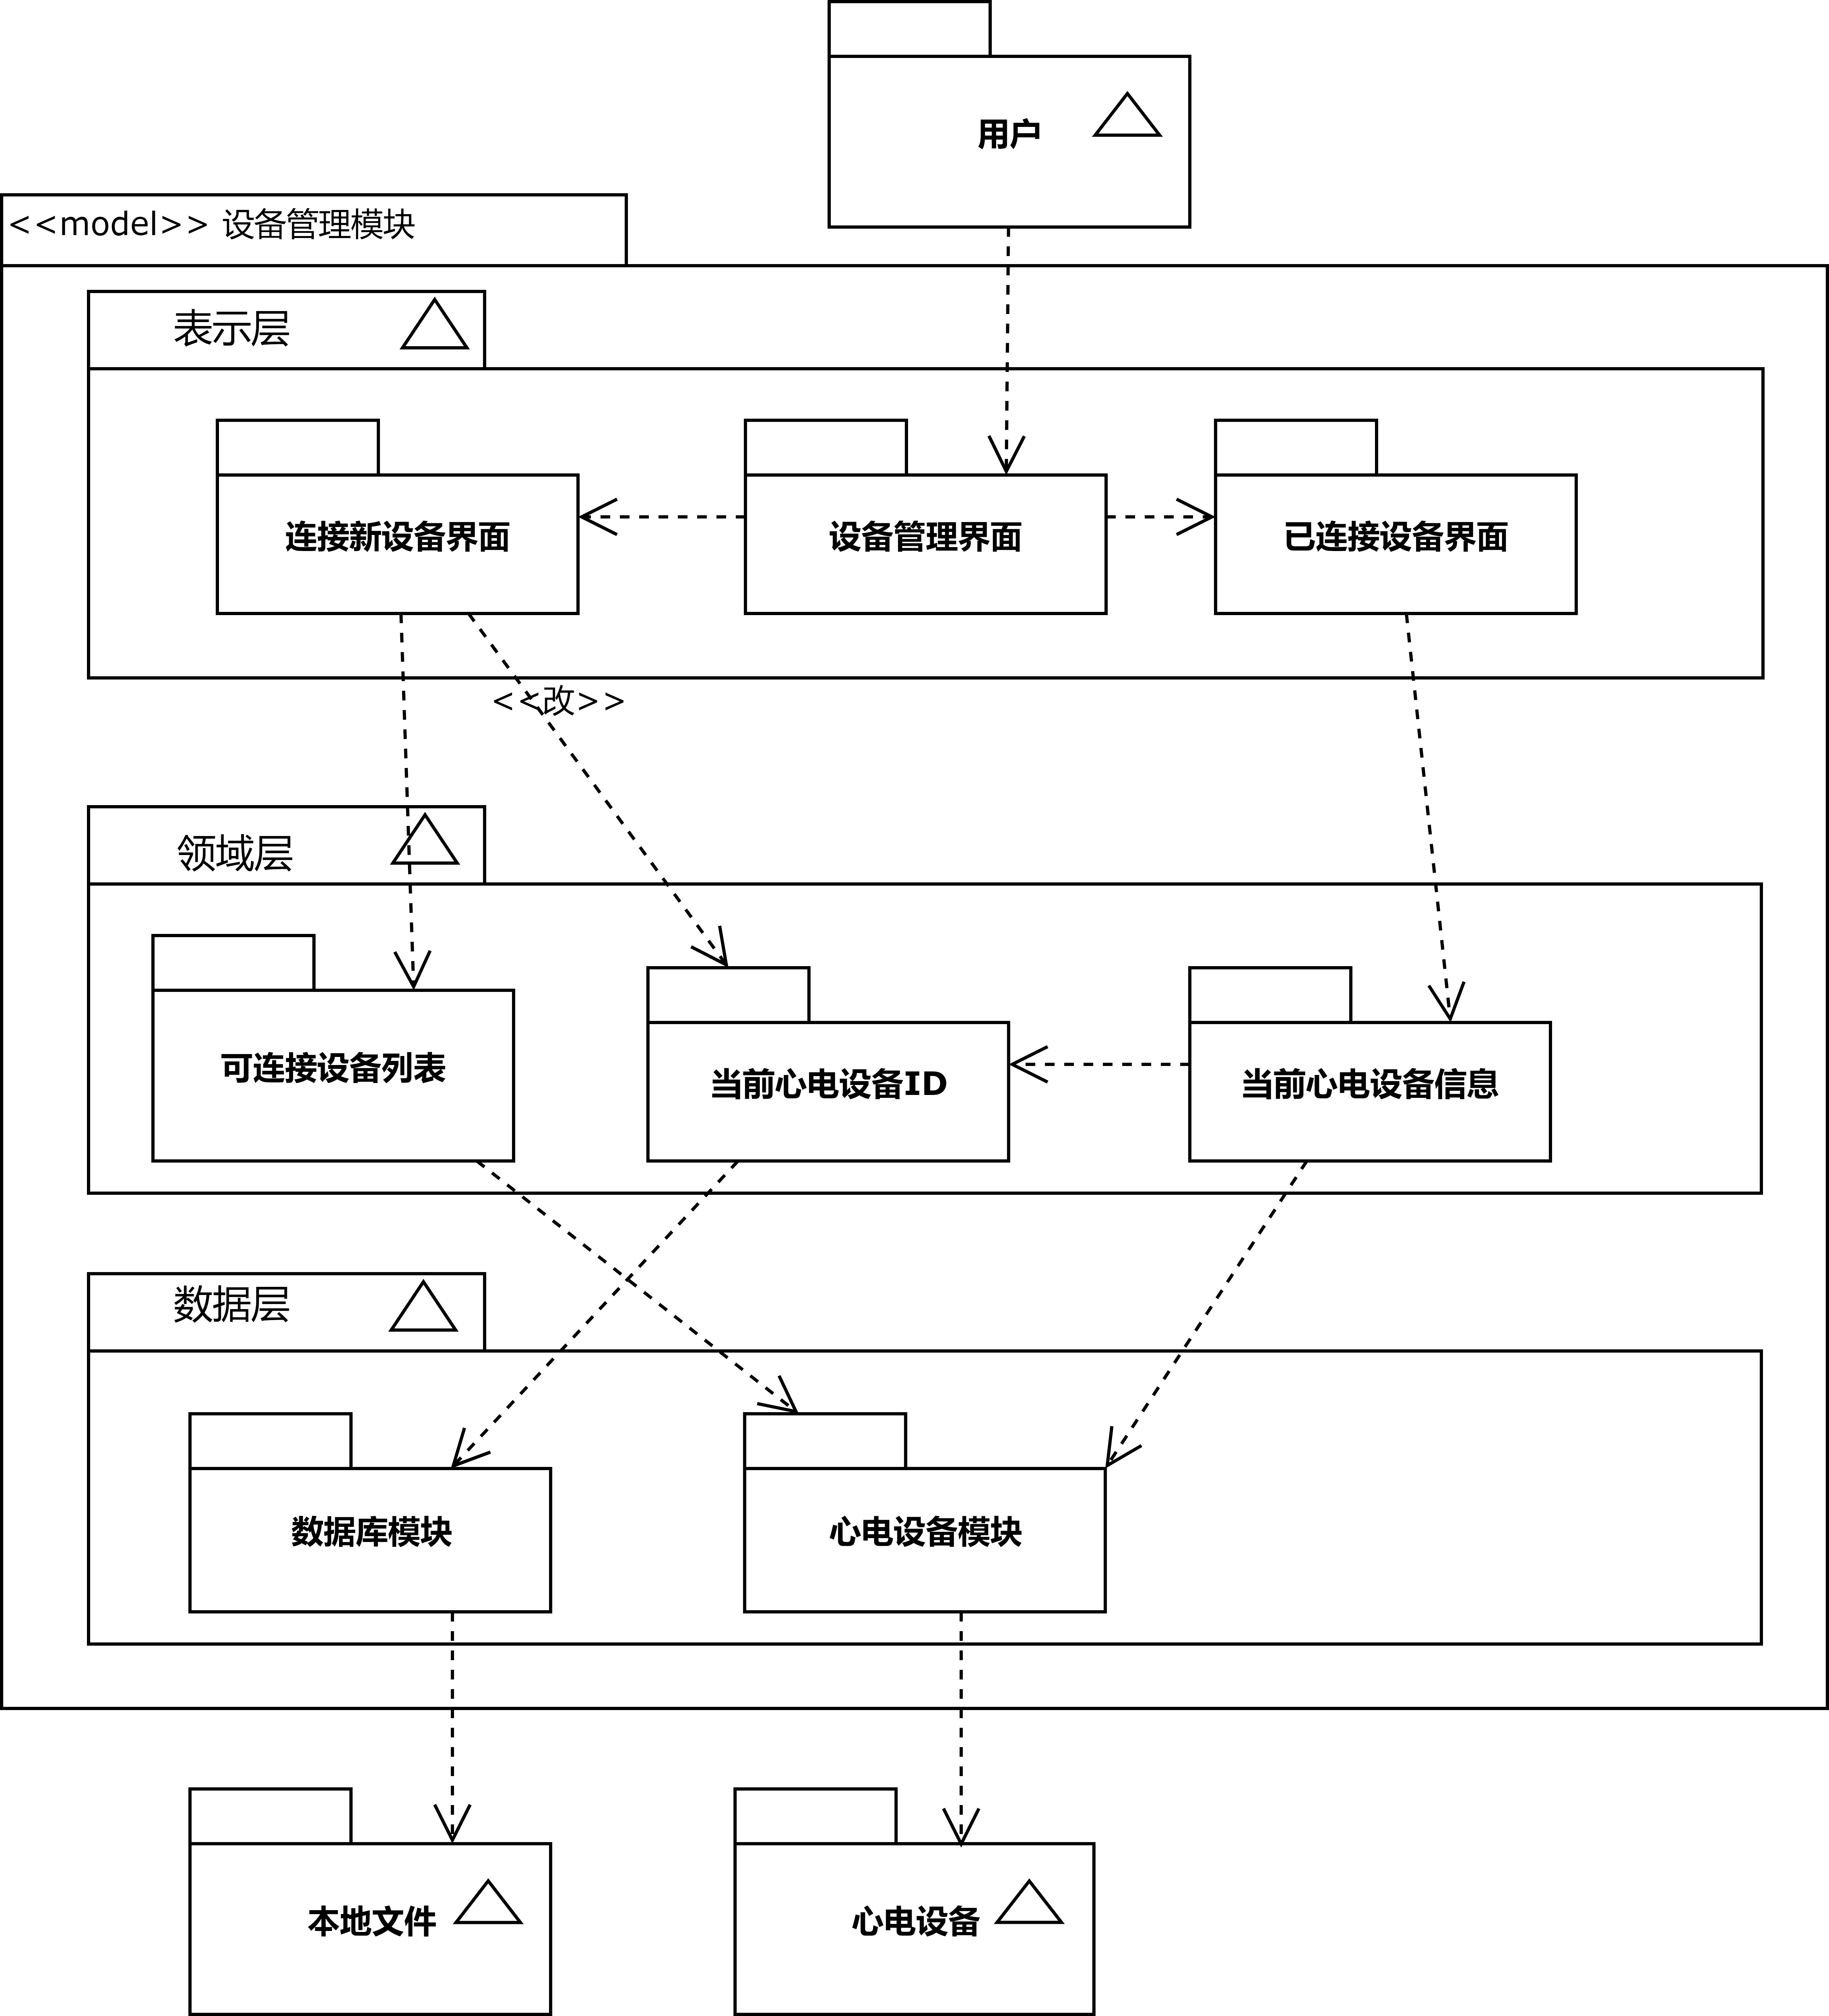
\includegraphics[width=.9\textwidth]{../assets/model-device.drawio}
    \bicaption{设备管理模块的架构}{Architecture of the device module}
    \label{fig:model-device}
\end{figure}

\subsubsection{表示层}

设备管理模块相比上述模块较为简单。虽然还有其他更简单的模块(如日志模块等),但因为在设计阶段几乎没有相关工作,故其他模块不在此章介绍。设备管理模块的表示层只包含一个面向用户的界面,即设备管理界面。设备管理界面实际上由两个不同的界面组成,在未连接设备的情况下是连接新设备界面,已连接设备的情况下则是已连接设备界面。由于两个界面的出现条件对立,因此将其合并为设备管理界面。在已连接设备界面中,点击解绑设备则会断开连接,切换至连接新设备界面。在连接新设备界面中,选择要连接的新设备则会进行连接,切换至已连接设备界面。

\subsubsection{领域层}

设备管理模块的领域层包含三个数据模型,即可连接设备列表、当前心电设备ID、当前心电设备信息。当前心电设备ID为字符串或 @null@,用于标识应用当前连接的设备,在应用程序启动时会从数据库读取,改变时也会写入数据库,设备管理界面在连接新设备界面和已连接设备界面之间的切换判定也是基于当前心电设备ID是否为 @null@。当前心电设备信息仅在心电设备已连接,即当前心电设备ID不为 @null@ 时有效,由已连接设备界面使用,其内容包括当前设备的信号强度、剩余电量等信息。可连接设备列表仅在连接新设备界面中有使用,为其提供可连接设备的名称与ID等信息,在连接后也会将所连接设备的ID更新至当前心电设备ID。

\subsubsection{数据层}

设备管理模块需要用到数据层中的数据库模块和心电设备模块。数据库模块用于连接的心电设备的ID的读写。心电设备模块用于与心电设备的通信和可供连接的设备的扫描。


\section{应用的数据库设计}\label{sec:db-design}

应用的数据库分为两部分,存储简单数据的SharedPreferences数据库和存储复杂数据的Isar数据库。前者主要用于存储应用的设置,后者主要用于存储历史心电数据与分析报告结果。

\subsection{SharedPreferences数据库的设计}\label{subsec:shared-preferences}

\subsubsection{SharedPreferences数据库介绍}\label{subsubsec:shared-preferences-intro}

SharedPreferences是Flutter的一个包,提供了简单键值对的存储功能,可以视为一个键值型的非关系型数据库。其在Android平台上基于同名的SharedPreferences功能,在iOS上则基于NSUserDefaults功能。

SharedPreferences仅支持少数几种数据类型,即 @int@、@double@、@bool@、@String@ 以及 @List<String>@。键值型数据库的读写非常简单,不需要进行特别的设计。本项目对该数据库的设计主要在于将各种需要存储的类型映射为其支持的类型。

\subsubsection{Duration类型的存储}\label{subsubsec:duration-storage}

Duration类型表示时间长度。由于应用内对时间的各种操作最多只需要毫秒精度,所以应用在需要将Duration类型的数据存入SharedPreferences时会将其转换为毫秒数以整数格式进行存储。在读取时,应用会将毫秒数转换为Duration类型。

\subsubsection{Color类型的存储}\label{subsubsec:color-storage}

Color类型表示颜色。应用在需要将Color类型的数据存入SharedPreferences时,会将其编码为32位整数以整数格式进行存储。在读取时,应用会将32位整数转换为Color类型。具体的编码方式是将颜色的ARGB值分别存储在32位整数的高8位、次高8位、次低8位和低8位中。

\subsubsection{枚举类型的存储}\label{subsubsec:enum-storage}

应用中使用了各种枚举类型,有时会需要将枚举类型存入SharedPreferences。应用在存储枚举类型时会将其转换为索引值,以整数形式存储。枚举类型常见的存储方式还包括按其名称以字符串形式存储、为每个枚举值赋予自定义值然后按自定义值的类型存储。相比其他方法,直接按索引值存储的优点在于其简单高效;缺点在于已经存在的枚举值不能轻易改动,否则会破坏已有的数据。由于应用内的枚举值设计基本不变,所以该缺点并不明显,可以接受。

\subsection{Isar数据库的设计}\label{subsec:isar}

\subsubsection{Isar数据库介绍}\label{subsubsec:isar-intro}

Isar是Flutter的一个包,提供了一个跨平台数据库。Isar属于非关系型数据库,不过提供了组合索引、ACID语义、事务等功能,可以视为一个关系型数据库的子集。相比常规的关系型数据库,Isar有一些额外的限制(或者说缺少一些功能)影响了本应用对数据库的设计。

当使用Isar来存储数据时,需要对Collection进行操作。Collection可理解为Isar数据库中的表,其包含的数据只能为同一类Dart对象,每个对象则代表了对应数据表中的一行数据。该类对象所对应的类则是这张表的Schema,其中每个字段对应数据库中的一列。与一般的关系型数据库相同的是,Schema中必须要有主键;不同的是,Isar中主键的类型被限制为64位整数值,这一限制导致了本应用对数据库的设计中的一些不同之处。

在查询时,Isar并不像一般的关系型数据库那样在编写SQL语句后自动生成最优查询策略,而是需要手动指定查询方式。Isar中的查询过滤方式分为两种,分别称为Filter和Where,前者执行遍历过滤,后者依靠索引表进行过滤。多个Where子句的过滤结果直接只能进行并集运算,无法进行交集运算。如果需要按多个属性进行过滤,并且还希望使用索引加快速度,就必须使用组合索引。组合索引有一个特殊的限制:主键不能包含在组合索引之中。这一限制也影响了本应用对数据库的设计。

此外,Isar对外键、Join等功能的支持也比较有限,不过这些功能在本应用的数据库设计中本来也不需要,所以不进行过多说明。

\subsubsection{心拍数据的存储}\label{subsubsec:beat-storage}

在分析报告数据中,只有心拍数据被存入数据库,基于心拍数据产生的进一步分析结果则只在查询时动态生成。这一方面是因为算法的大部分时间开销在于分割分类模型的运行上,其余部分开销较小。另一方面是因为心拍之外的结果的格式较为复杂,不方便进行合适的数据库设计。心拍数据则格式简单,且存储、查询时可以对多段数据进行拼接、裁剪而不失去太多准确度,所以适合存入数据库之中。

心拍数据的Schema包含3个字段和2个索引。字段中的ID是由Isar管理的自增整数,没有特别用途。另外两个字段分别是DateTime类型的心拍时间和枚举类型的心拍类型标签。对心拍时间进行了单列索引,以方便在查看历史心电时快速检索指定时间范围内的所有心拍。对心拍类型和心拍时间进行了组合索引,以心拍类型为主索引,这个组合索引用于查询指定标签在指定时间范围内的数量等信息。

\subsubsection{心电数据的存储}\label{subsubsec:point-storage}

对心电数据的查询需求较为简单,只有在历史心电界面中需要对指定时间范围内的心电数据进行查询。因此,也只需要在心电数据的时间上进行索引。

由于没有组合索引的需求,所以可以直接把时间作为主键,以节省额外的索引表的开销,并避免浪费主键所占的空间。由于主键只能为64位整数,所以需要对时间进行编码。考虑到时间只需要毫秒精度,将其编码为了自Unix纪元(UTC时间的1970年1月1日00:00:00)以来经过的毫秒数。这样,心电数据的Schema中不包含任何额外定义的索引,查询时只使用主键自带的索引功能。

除了作为主键的时间之外,一条心电数据中还包含各导联的电压数据。由于导联I、II、III被定义为左臂、右臂、左腿三个点之间的电位差,这三个导联的数据实际上只包含两个差值的信息量,所以只需要存储两个值即可。
